% Pictorial scenes and native drawings share the essay's caption treatment.
\newcommand{\EssayIllustration}[4]{%
  \par
  \begin{center}
    \begin{minipage}{\linewidth}\centering
    \includegraphics[width=\linewidth,height=#2,keepaspectratio]{#1}\par
    \captionof{figure}{#3}\label{#4}
    \end{minipage}
  \end{center}\par
}
\newcommand{\WideEssayIllustration}[4]{%
  \begin{center}
    \begin{minipage}{\textwidth}\centering
    \includegraphics[width=0.94\textwidth,height=#2,keepaspectratio]{#1}\par
    \captionof{figure}{#3}\label{#4}
    \end{minipage}
  \end{center}
}

\newcommand{\FactoryRetrofitArt}{%
  \WideEssayIllustration{factory-retrofit-v2.png}{54mm}
    {Illustrative retrofit: a new power source can leave the inherited production layout intact.}
    {fig:factory-retrofit}%
}
\newcommand{\CoInventionArt}{%
  \WideEssayIllustration{co-invention-workshop-v2.png}{115mm}
    {Co-invention develops the operating use alongside the mechanism: meanings, permitted actions, and acceptance must become workable together.}
    {fig:co-invention}%
}
\newcommand{\FragmentedAssignmentArt}{%
  \EssayIllustration{fragmented-assignment.png}{48mm}
    {Being fully occupied does not establish an assignment for the integrated scope a producer can carry.}
    {fig:fragmented-assignment}%
}
\newcommand{\ComplementaryAssetsArt}{%
  \WideEssayIllustration{complements-operating-access-v2.png}{78mm}
    {A commission becomes operable through contributions held by different parties: the customer's mandate, the interface provider's access, and the factory owner's capacity commitment.}
    {fig:complements}%
}
\newcommand{\ReusableCoInventionArt}{%
  \WideEssayIllustration{reusable-co-invention.png}{78mm}
    {A later application can inherit tested methods and operating knowledge; its local facts and authority must still be established.}
    {fig:reusable-co-invention}%
}
\newcommand{\HandoverArt}{%
  \par\smallskip\noindent
    \begin{minipage}{\textwidth}\centering
    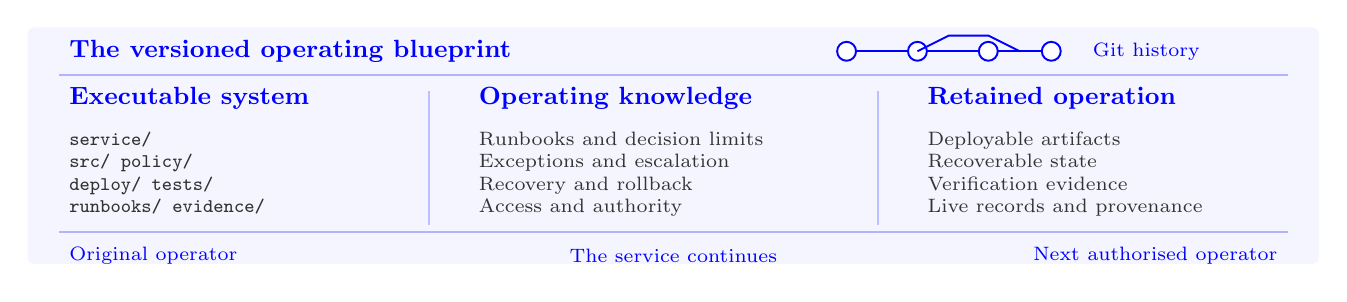
\begin{tikzpicture}[x=1mm,y=1mm,draw=blue,text=blue,line width=0.7pt]
      % The same retained system is usable across an operator change.
      \fill[blue!4,rounded corners=2pt] (0,0) rectangle (164,30);
      \node[anchor=west,font=\small\bfseries] at (4,27) {The versioned operating blueprint};
      \draw (104,27)--(130,27);
      \foreach \xx in {104,113,122,130}
        \draw[fill=white] (\xx,27) circle (1.2);
      \draw (113,27)--(117,29)--(122,29)--(126,27);
      \node[anchor=west,font=\scriptsize] at (134,27) {Git history};
      \draw[blue!30] (4,24)--(160,24);
      \node[anchor=west,font=\small\bfseries] at (4,21) {Executable system};
      \node[anchor=north west,align=left,font=\scriptsize\ttfamily,text=black!80]
        at (4,18) {service/\\src/ policy/\\deploy/ tests/\\runbooks/ evidence/};
      \draw[blue!25] (51,5)--(51,22) (108,5)--(108,22);
      \node[anchor=west,font=\small\bfseries] at (56,21) {Operating knowledge};
      \node[anchor=north west,align=left,font=\scriptsize,text=black!80]
        at (56,18) {Runbooks and decision limits\\Exceptions and escalation\\Recovery and rollback\\Access and authority};
      \node[anchor=west,font=\small\bfseries] at (113,21) {Retained operation};
      \node[anchor=north west,align=left,font=\scriptsize,text=black!80]
        at (113,18) {Deployable artifacts\\Recoverable state\\Verification evidence\\Live records and provenance};
      \draw[blue!30] (4,4)--(160,4);
      \node[anchor=west,font=\scriptsize] at (4,1) {Original operator};
      \node[font=\scriptsize] at (82,1) {The service continues};
      \node[anchor=east,font=\scriptsize] at (160,1) {Next authorised operator};
    \end{tikzpicture}\par
    \captionof{figure}{Continuity resides in a versioned operating blueprint: executable code, runbooks, deployable artifacts, recoverable state, and verification evidence that another authorised operator can use.}
    \label{fig:handover}
    \end{minipage}
  \par\smallskip%
}

% Three ordinary objects distinguish measurement questions without invented data.
\newcommand{\MeasurementArt}{%
  \par
  \begin{center}
    \begin{minipage}{\linewidth}\centering
    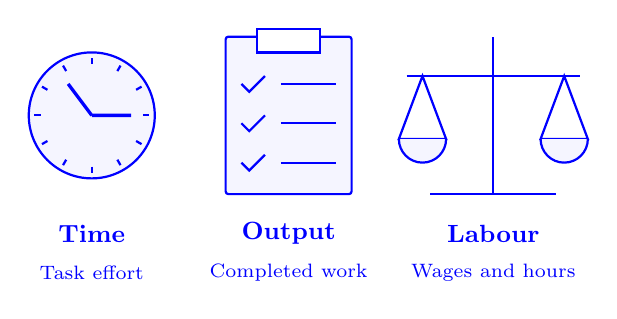
\begin{tikzpicture}[x=1mm,y=1mm,draw=blue,text=blue,line width=0.8pt]
      \draw[fill=blue!4] (12,16) circle (8);
      \foreach \angle in {0,30,...,330}
        \draw[shift={(12,16)}] (\angle:6.5)--(\angle:7.3);
      \draw[line width=1.2pt] (12,16)--(9,20) (12,16)--(17,16);
      \node[font=\small\bfseries] at (12,1) {Time};
      \node[font=\scriptsize] at (12,-4) {Task effort};
      \draw[fill=blue!4,rounded corners=1pt] (29,6) rectangle (45,26);
      \draw[fill=white] (33,24) rectangle (41,27);
      \foreach \yy in {20,15,10} {
        \draw (31,\yy)--(32,\yy-1)--(34,\yy+1);
        \draw (36,\yy)--(43,\yy);
      }
      \node[font=\small\bfseries] at (37,1) {Output};
      \node[font=\scriptsize] at (37,-4) {Completed work};
      \draw (63,6)--(63,26) (55,6)--(71,6) (52,21)--(74,21);
      \draw (54,21)--(51,13)--(57,13)--cycle;
      \draw (72,21)--(69,13)--(75,13)--cycle;
      \draw[fill=blue!4] (51,13) arc (180:360:3);
      \draw[fill=blue!4] (69,13) arc (180:360:3);
      \node[font=\small\bfseries] at (63,1) {Labour};
      \node[font=\scriptsize] at (63,-4) {Wages and hours};
    \end{tikzpicture}\par
    \captionof{figure}{Different measures observe different changes; they do not supply one interchangeable estimate of AI's economic effect.}
    \label{fig:measurement}
    \end{minipage}
  \end{center}\par
}

% A conceptual floor plan for the quotation example, rather than a flowchart.
\newcommand{\RecompositionArt}{%
  \begin{center}
    \begin{minipage}{\textwidth}\centering
    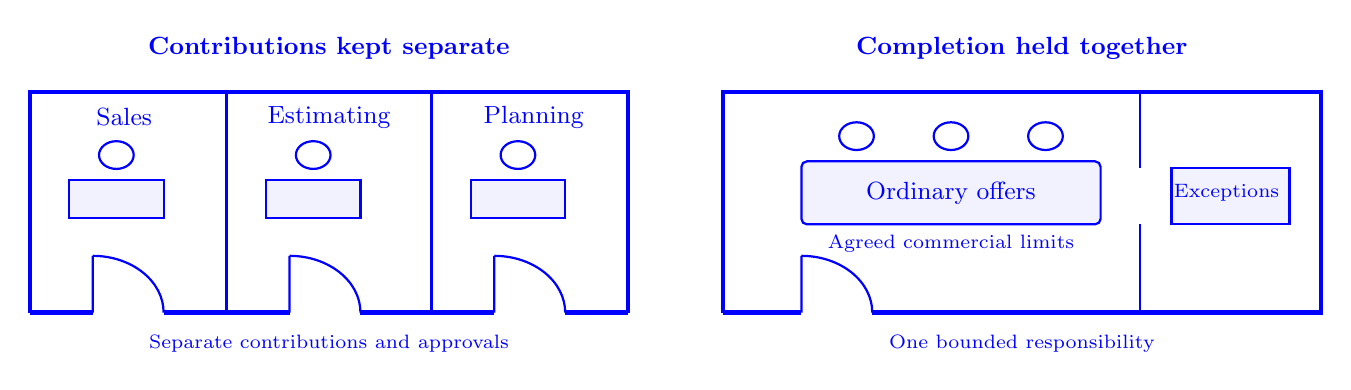
\begin{tikzpicture}[x=1mm,y=0.80mm,draw=blue,text=blue,line width=0.8pt]
      \node[font=\small\bfseries] at (38,47) {Contributions kept separate};
      \node[font=\small\bfseries] at (126,47) {Completion held together};
      \draw[line width=1.5pt] (0,5)--(0,40)--(76,40)--(76,5);
      \draw[line width=1.5pt] (0,5)--(8,5) (17,5)--(33,5) (42,5)--(59,5) (68,5)--(76,5);
      \draw[line width=1.2pt] (25,5)--(25,40) (51,5)--(51,40);
      \foreach \xx in {8,33,59} {
        \draw (\xx,5)--(\xx,14) (\xx,14) arc (90:0:9);
        \draw[fill=blue!5] (\xx-3,20) rectangle (\xx+9,26);
        \draw[fill=white] (\xx+3,30) circle (2.2);
      }
      \node[font=\small] at (12,36) {Sales};
      \node[font=\small] at (38,36) {Estimating};
      \node[font=\small] at (64,36) {Planning};
      \node[font=\scriptsize] at (38,0) {Separate contributions and approvals};
      \draw[line width=1.5pt] (88,5)--(88,40)--(164,40)--(164,5)--(107,5);
      \draw[line width=1.5pt] (88,5)--(98,5);
      \draw (98,5)--(98,14) (98,14) arc (90:0:9);
      \draw[fill=blue!5,rounded corners=2pt] (98,19) rectangle (136,29);
      \foreach \xx in {105,117,129} \draw[fill=white] (\xx,33) circle (2.2);
      \node[font=\small] at (117,24) {Ordinary offers};
      \node[font=\scriptsize] at (117,16) {Agreed commercial limits};
      \draw (141,5)--(141,19) (141,28)--(141,40);
      \draw[fill=blue!5] (145,19) rectangle (160,28);
      \node[font=\scriptsize] at (152,24) {Exceptions};
      \node[font=\scriptsize] at (126,0) {One bounded responsibility};
    \end{tikzpicture}\par
    \captionof{figure}{Quotation recomposition: we predict lower coordination costs, earlier usable offers, and more small or variable orders becoming economical to serve \citep{milgrom1995complementarities,dellacqua2026teammate}.}
    \label{fig:recomposition}
    \end{minipage}
  \end{center}
}
